\section{Incentivization Mechanism}
\label{sec:incentiviationmechanism}

The HOPR protocol provides incentives to nodes in the network to achieve correct
transformation and delivery of mixnet packets. This is accomplished through a
combination of \textbf{Proof-of-Relay}, a novel mechanism which is
cost-effective and privacy-preserving, and \textbf{Probabilisitic Payments}.
While the high-level overview of the incentives has been covered in the
\nameref{sec:introduction}, this section focuses on the technical details which
are used to realize the mechanism.

\subsection{Probabilistic Payments}

In traditional payment channels, two parties A and B lock some funds within a
smart contract, make transactions off-chain and only commit the aggregation
on-chain. Thus, a channel is bidirectional which means that both A and B can
send and receive transactions within the same channel. The HOPR protocol uses
unidirectional channels where the channel creator is the sole owner of
funds in the channel and the one able to create tickets. A channel created from
party $A$ to party $B$ is different from a channel created from party $B$ to
party $A$.

 $$A\rightarrow B \neq B\rightarrow A$$
This separation reflects the directional nature of packets flowing through the
network.
\\\textbf{Acknowledgements} are messages which allow every node to acknowledge the
processing of a packet to the previous node. This acknowledgement contains the
cryptographic material to unlock the possible payout for the previous node. Note
that acknowledgement is always sent to the previous node.
\\An acknowledgement contains all previous incentives plus the incentive for the
most recent interaction.

\begin{align}
value_(ACK_n) &=\sum_{i=1}^nfee_{packet_i}
\end{align}
where $n$ is the total number of mixnet packets transformed.
\\If B received $ACK_n$ for $packet_n$ before sending $packet_{n-1}$, it has no
incentive to process $packet_{n-1}$ rather than $packet_{n}$. To avoid these
false incentives the HOPR protocol utilizes \textbf{probabilistic payments}.
In probabilistic payments the payouts use \textit{tickets} (further explained in
section \nameref{sec:tickets}). A ticket can be either a win or a loss with a
certain winning probability. This means nodes are incentivized to continue
relaying packets as they don’t know which ticket is a win. To a node each
ticket has the same value it is being claimed, thus the HOPR protocol
encourages nodes to claim tickets independently from each other.

\begin{align}
 value ( ACK_i )  &  =value ( ACK_j ) \quad for \quad i,j\in \{1,n\}
\end{align}
There is no added value in pretending packet loss or intentionally changing the order in which packets are processed.

\subsubsection{Channel Management}
Initially, each payment channel in HOPR is CLOSED which means that in order to transfer packets, those channels have to be opened. There are four distinct channel statuses which are represented in the following scheme:

\begin{figure}[H]
    \centering
    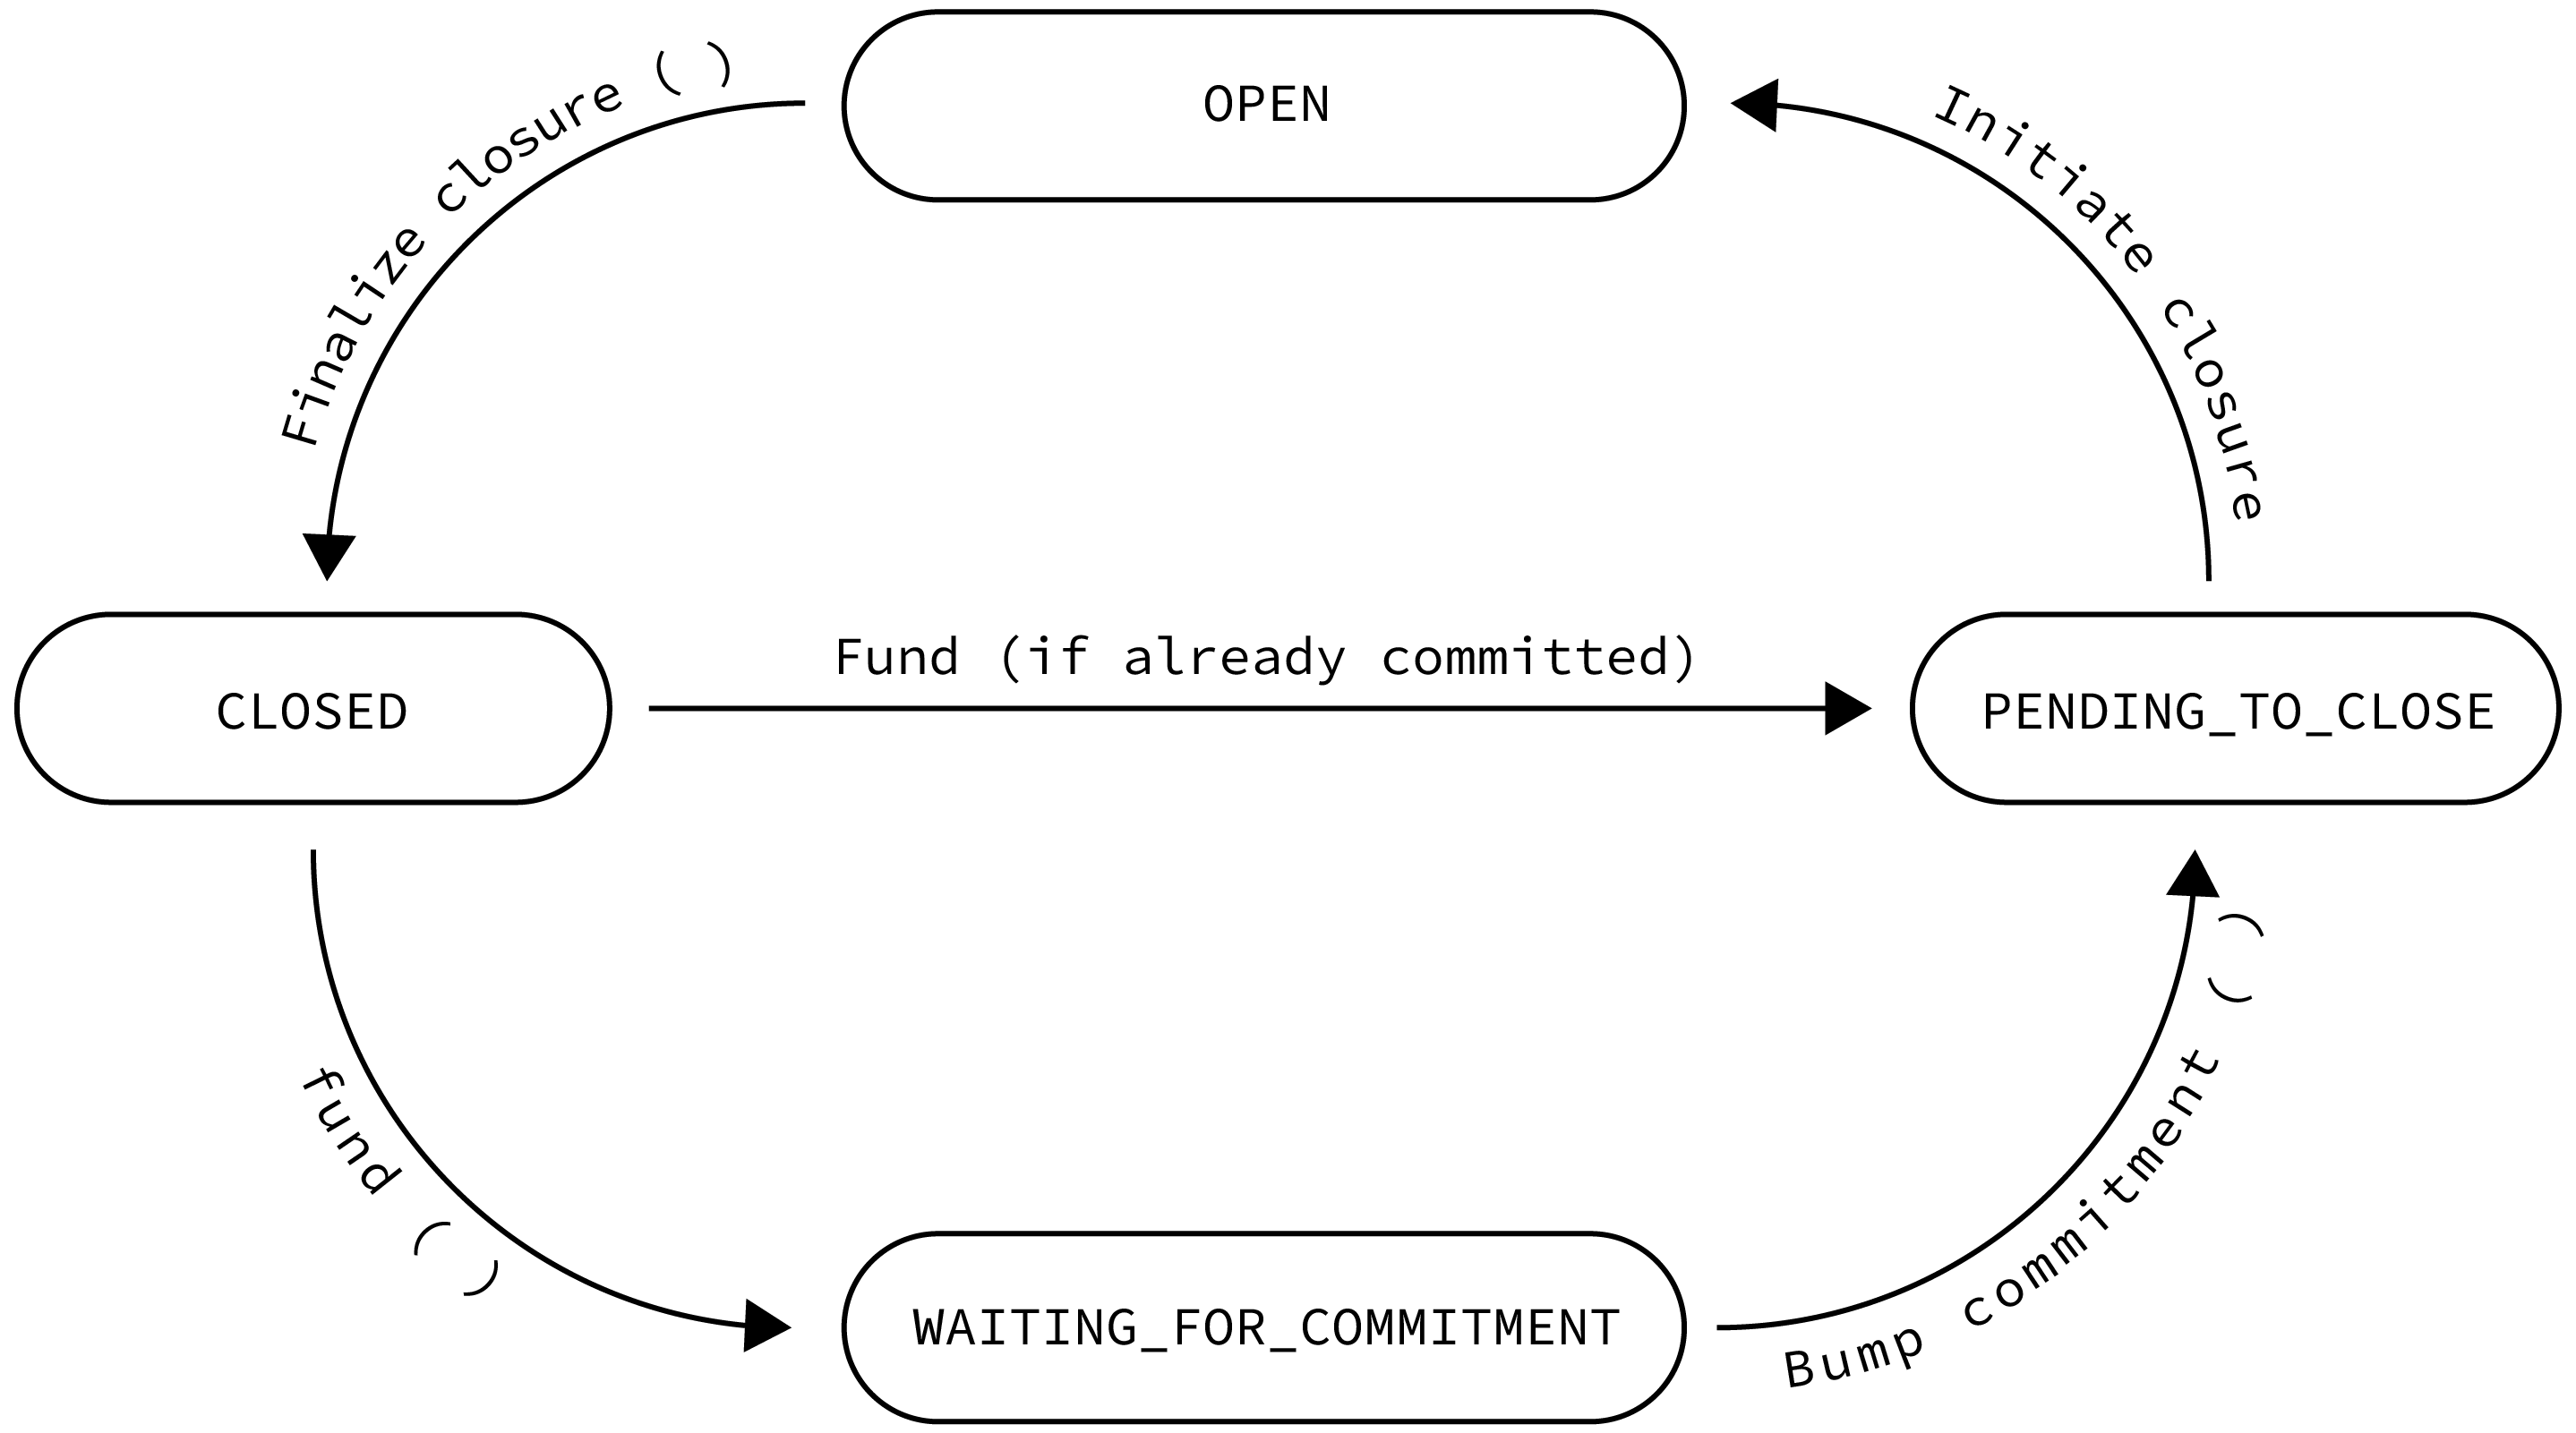
\includegraphics[width=9cm,height=9cm,keepaspectratio]{../yellowpaper/images/states1.png}
\label{fig:channel statuses}
    \caption{Channel statuses}
\end{figure}

\paragraph{Opening a channel} Nodes can OPEN channels to other nodes by the following:
A calls the method \textit{fundChannelMulti()} such that:
$$fundChannelMulti(A: <\lambda>, B:<\mu> )$$ where $\lambda$ and $\mu$ are the amounts to be staked by the sender A for A and B. Both values can also be equal or any of them could be zero. This function opens two unidirectional channels $A\rightarrow B$ and $B\rightarrow A$ if both staked amounts are specified. If not, only the channel $A\rightarrow B$ is opened where $A$ is the sender and $B$ is the recipient.
The channel is then on state \textit{WAITING\_FOR\_COMMITMENT}.
\\~\\The destination address of the channel must now commit in order for the channel between both parties to be open.
The channel destination (let's say it's B) can now call \textit{bumpChannel()} function to make a new set of commitments towards this channel. This call will trigger an onchain event \textit{ChannelIsOpened} and bumbs the ticket epoch to ensure tickets with the previous epoch are invalidated

\paragraph{Redeem tickets}
As long as the channel remains open, nodes can claim their incentives for forwarding packets which is represented as tickets (see ticket section). Tickets are redeemed by dispatching a \textit{redeemTicket()} call.
\\~\\If/when B tries to redeem a ticket from the channel $A\rightarrow B$ (spending channel) but also there is an open channel $B\rightarrow A$ (earning channel), B's rewards will go to $B\rightarrow A$. Otherwise, rewards will be sent directly to B.

\paragraph{Closing a channel}
Nodes can close a payment channel in order to access their funds. The way to do so is using a timeout.
Only the channel creator (let's say it's A) can initiate the process by calling \textit{initiateChannelClosure()}. This changes the state to $PENDING\_TO\_CLOSE$. Other nodes should monitor blockchain events to be aware of this change and thus will have now time to claim not yet claimed tickets.
\\~\\Once the timeout is done, (A) can call \textit{finalizeChannelClosure()} which turns the channel state into CLOSED. When channel is closed, funds (stake) are transfered automatically back to (A). Every ticket that wasn't redeemed while channel was open can't be redeemed after closure. This is guaranteed by using Channel Epoch which is explained in ticket section.

\begin{comment}

\begin{figure}[H]
    \centering
    \begin{tikzpicture}[looseness=1,auto]
        \path (0,0) node (closed) [ellipse,draw] {$Closed$};
        \path (-1,-1)  node (commitment) [ellipse,draw,align=left] {$Waiting$\\$Commitment$};
        \path (5,0)  node (open) [ellipse,draw] {$Open$};
        \path (2.5,-1)  node (pending) [ellipse,draw,align=left] {$Pending$\\$Timeout$};

        \draw [->,draw](closed) to [bend left] node {\textsf{fund()}} (commitment);
        \draw [->,draw](commitment) to [bend left] node {\textsf{fund()}} (open);
        \draw [->,draw](open) to [bend left] node [align=center] {\textsf{initiateChannelClosure()}} (pending);
        \draw [->,draw](pending) to [bend left] node {\textsf{finalizeChannelClosure()}} (closed);

        \path[->] (open) edge [out=+120,in=+60,distance=2em,below] node [align=center,above] {\textsf{redeemTicket()}}  (open);
    \end{tikzpicture}
    \label{fig:channel workflow}
    \caption{Channel workflow}
\end{figure}
\end{comment}

\begin{comment}
  \draw [->,draw](commitment) to [bend left] node {\textsf{fund()}} (open);
    \draw [->,draw](open) to [bend left] node [align=center] {\textsf{initiateChannelClosure()}} (pending);
    \draw [->,draw](pending) to [bend left] node {\textsf{finalizeChannelClosure()}} (closed);  
\end{comment}


\subsection{On-chain Commitment}

HOPR uses a commitment scheme to deposit values on-chain and reveal them once a node redeems an incentive for relaying packets. This comes with the benefit that the redeeming party discloses a secret that is unknown to the issuer of the incentive until it is claimed on-chain. The $opening$ and the $response$ to the PoR challenge are then used by the smart contract to determine whether the ticket has been redeemed or not.

\begin{defnsub}
    % Currently leaving out further details such as unconditionally/computationally binding / hiding
    A commitment scheme $Cm = (\mathsf{Commit}, \mathsf{Open})$ is a protocol between two parties, $A$ and $B$, that gives $A$ the opportunity to store a value $comm = \mathsf{Commit}(x)$ at $B$. The value $x$ stays unknown to $B$ until $A$ decides to reveal it to $B$.

    \noindent\textbf{Hiding:} A commitment scheme is called \textbf{hiding} if it is infeasible for an adversary $\mathsf{Adv}$ to recover $x$ from $comm$.

    \noindent\textbf{Binding:} A commitment scheme is called \textbf{binding} if it is infeasible for an adversary $\mathsf{Adv}$ to find a value $x'$ with $x \neq x'$ such that $\mathsf{Open}(cm, x') \neq \bot$.
\end{defnsub}

\subsubsection{Setup phase}

Once a node engages with another node in a payment channel and lock funds within that channel, it derives a master key $comm_0$ from its private key and uses it to create an iterated commitment $comm_i$ such that for every $i \in \mathbb{N}_0$ and $i > 0$ it holds that $$ \mathsf{Open}(comm_{i}, comm_{i-1}) = \top $$
The iterated commitment is computed as $$comm_n = hash^n(comm_0)$$ where $\mathsf{hash}$ is a preimage-resistant hash function and $comm_0$ is derived as 
$$ comm_0 = \mathsf{hash}(privKey, chainId, contractAddr, channelId, channelEpoch)$$
The master key is supposed to be pseudo-random such that all intermediate commitments $comm_{i}$ for $i \in \mathbb{N}_0$ and $0 < i \le n$ are indistinguishable for the ticket issuer from random numbers of the same length. This is necessary in order to ensure that the ticket issuer is unable to determine whether a ticket is a win or not when issuing the ticket. This makes it infeasible for the ticket issuer to tweak the challenge to such that it cannot be a win.
\\~\\When dispatching a transaction that opens the payment channel, the commitment $comm_n$ is stored in the channel structure in the smart contract and the smart contract will force the ticket recipient to reveal $comm_{n-1}$ when redeeming a ticket issued in this channel.
The number of iterations $n$ can be chosen as a constant and should reflect the number of tickets a node intends to redeem within a channel.

\subsubsection{Opening phase}

In order to redeem a ticket, a node has to reveal the opening to the current commitment $comm_i$ that is stored in the smart contract for the channel. Since the opening $comm_{i-1}$ allows the ticket issuer to determine whether a ticket is going to be a win, the ticket recipient should keep $comm_{i-1}$ until it is used to redeem a ticket.
Tickets lead to a win if $\mathsf{hash}( t_h, r, comm_{i-1} ) < P_w$ where $t_h=\mathsf{hash}(t)$ and $\mathsf{Open}(comm_i, comm_{i-1}) = \top$. Since $comm_{0}$ is known to the ticket recipient, the ticket recipient can compute the opening as $comm_{n-1} = \mathsf{hash}^{n-1}(comm_0)$.
Once redeeming a ticket, the smart contract verifies that $$\mathsf{Open}(comm_i, comm_{i-1}) = \top$$ and sets $channel.comm[redeemer] \leftarrow comm_{i-1}$. Hence next time, the node redeems a ticket, it has to reveal $comm_{i-2}$.
In addition, each node is granted the right to reset the commitment to a new value which is necessary especially once a node reveals $comm_0$ and therefore is with high probability unable to compute a value $r$ such that $$\mathsf{Open}(comm_0,r) \neq \bot$$
Since this mechanism can be abused by the ticket recipient to tweak the entropy that is used to determine whether a ticket is a win or not, the smart contract keeps track on resets of the on-chain commitment and sets $$channel.ticketEpoc[redeemer] \leftarrow channel.ticketEpoc[redeemer] + 1$$ and thereby invalidates all previously unredeemed tickets.




\subsection{Proof Of Relay}
\label{sec:proofofrelay}

HOPR incentivizes packet transformation and delivery using a mechanism called
“Proof-Of-Relay”. This mechanism guarantees that nodes relay services are
verifiable.

\paragraph{Construction}
\begin{itemize}
    \item Every packet is sent together with a ticket (check ticket section).
    \item Each ticket contains a challenge.
    \item The validity of a ticket can only be checked on reception of the packet but the on-chain logic enforces a solution to the challenge stated in the ticket (check ticket section).
\end{itemize}

\subsubsection{Challenge}

$(A)$ creates a shared group element $\alpha_i$ with all the relay nodes in the channel (B-C-D-Z) by using an offline version of the Diffie-Hellman key exchange. This shared key is a session key that's generated from the master DH sphinx key and will be used to derive new keys $s_i^{(0)}$ and $s_{i}^{(1)}$. 
The first key $s_i^{(0)}$ will be used as the node's \textit{own key share} and the second key $s_i^{(1)}$ will be used as the \textit{acknowledgement key} which will be embedded in the acknowledgement for a packet and thereby unlocks the incentive for the previous relayer for transforming and delivering the packet.
    \paragraph{Key derivation}
    We first create a "session secret" $s_i$ then we use it as a seed to derive subkeys $s_i^{(0)},s_i^{(1)}$ for each node on the route. We do so using a HKDF (HMAC-based Key Derivation Function) which is a cryptographic hash function that derives one or more secret keys from a secret value using a pseudorandom function. The key derivation works as follows:
    \begin{itemize}
        \item Extract: Creates a pseudo-random key $s_i$   
        $$HKDF.extract(h_b, |h_b|, \alpha_i* privKey || pubKey)$$   

        \item Expand: This step takes the output of the previous one $s_i$ as a seed and creates an output key material $s_i^{(0)},s_i^{(1)}$ which is expanded from hashes of $s_i$ and an optional info message (salt). The process goes as follows:
        $$HKDF.expand(h_b, |h_b|,s_i, |s_i|, hashKey)$$
    \end{itemize}
    where $||$ is concatenation and $*$ is scalar multiplication on the curve. $h_b$ is blake2s256 hash algorithm, $|h_b|$ is its length, $s_i$ is the pseudo random key used as a seed and $|s_i|$ is its length, $hashKey$ is an identifier used to create a "virtual" hash function for each purpose, e.g. for the PRG, one for PRP, etc. and as well as for the PoR scheme. In case the result of HKDF does not lead to a field element, $hashKey$ is padded until that's the case.
    \\~\\ The sender $(A)$ provides a hint to the expected value $s_{i+1}^{(1)}$ that a node $n_i$ is expected to get from the next downstream node.
    The value “hint” or $H$ is computed as 
    \begin{align}  
        H_i&=s_{i+1}^{(1)}*G
         \end{align}
    where $*$ is the curve multiplication operation and $G$ is a generator of the curve (the same used in the sphinx section). 
    \newline The hint for party $n_i$ is used to check whether the returned value $s_{i+1}'^{(1)}$ matches the promised value $s_{i+1}^{(1)}$ by checking whether $H_i$ equals $s_{i+1}'^{(1)}*G$. 
   \\The sender $(A)$ also creates a challenge $T_{c_i}$ such that 
   \begin{align}  
    T_{c_i}&=(s_i^{(0)}+s_{i+1}^{(1)})*G
     \end{align}
   Since “Proof-Of-Relay” is used to make the relay services of nodes verifiable, it is the duty of each node to check that given challenges are derivable from the given and the expected information.
Packets with inappropriate challenges should be dropped as they might not lead to winning tickets.
\\The values $H_i$ and $T_{c_i}$ are sent with the routing information $\beta_i$ as follows:
$$\beta_i=y_{i+1}\|H_i\|T_{c_i}\|\gamma_{i+1}\|\beta_{{i+1}_{[ \,0....(2r-1)\kappa-1\,] }}\oplus \rho(h_{\rho}(s_{i}))_{[ \,0....(2r+1)\kappa-1\,]}$$
By decrypting $\beta_i$, each mix node $n_i$ will retrieve the public key of the next downstream node and both the hint and challenge which will be used in the Proof Of Relay to make sure relay services are verifiable.

\begin{comment}
 \begin{figure}[H]
    \centering
    \begin{tabular}{| m{2em} | m{15em} | m{2em} |}
        \hline
        $\alpha$ & $\beta$                   & $\gamma$ \\
                 & \begin{tabular}{| c m{2em} | m{3em} | m{6em} |}
            \hline
            \multicolumn{2}{| c |}{$Y_B$} & $hint_B$                 & $challenge_{BC}$ \\
            \hline
            \multicolumn{2}{| c |}{$Y_C$} & $hint_C$                 & $random$         \\
            \hline
            \multicolumn{2}{| c |}{$Y_D$} & $hint_D$                 & $random$         \\
            \hline
            End                           & \multicolumn{3}{| l |}{}                    \\
            \hline
        \end{tabular} &          \\[3em]
        \hline
    \end{tabular}
    \caption{Sphinx with PoR}
    \label{fig:Sphinx with PoR}
\end{figure}
\end{comment}

